\documentclass[a4paper]{article}
\usepackage{fixltx2e}
\usepackage{INTERSPEECH2018}

\title{A New Method for Monaural Speech Separation using Ideal Binary Mask}
\name{M. Naveen Narayanan$^1$, S. Somasundar$^1$, R. Rajavel$^2$, S. Sivakumar$^3$}
%The maximum number of authors in the author list is twenty. If the number of contributing authors is more than twenty, they should be listed in a footnote or in acknowledgement section, as appropriate.
\address{
  $^1$Undergraduate Students, SSN College of Engineering\\
  $^2$Associate Professor, SSN College of Engineering\\
	$^3$Associate Professor, JPR-SRR College of Engineering}
\email{rajavelr@ssn.edu.in, sivacud@gmail.com}

\begin{document}

\maketitle
% 
\begin{abstract}
  This research work proposes a new computationally efficient method for monaural speech separation using Ideal Binary Mask (IBM). Speech separation systems using IBM in general consists of time-frequency (T-F) analysis by a bank of Gamma tone analysis filters, ideal binary mask computation using clean speech and noise and finally reconstruction of speech using the computed IBM via synthesis filter bank. This method involves post multiplication of IBM with the output of the synthesis filter bank. Which involves many computations without contributing anything to the final output with increased computational delay. This research work solves this issue by changing the order of operation in the reconstruction of speech signal from the noisy speech and improves the performance with minimal computational delay. The proposed method multiplies the computed IBM with T-F signals from the output of the analysis filter bank. This in turn makes many noise dominant frames to be zeros and enables the synthesis filter bank to produce the enhanced speech signal with minimal computational delay. The experimental results show that the proposed approach improves the intelligibility and quality of speech in terms of Short Time Objective Intelligibility (STOI) and Signal to Noise Ratio (SNR) respectively. The proposed method also reduces the computation time considerably as compared to the existing approach of monaural speech separation.


\end{abstract}
\noindent\textbf{Index Terms}: Monaural speech separation - Ideal Binary Mask (IBM) – Gamma tone filter bank - Short Time Objective Intelligibility (STOI) – Signal to Noise Ratio (SNR)

\section{Introduction}

Monaural speech separation is a challenging signal processing problem that finds a lot of applications in speech processing such as speech/speaker recognition, voice communication, air-ground communication and hearing aids. Over the last few decades, researchers have proposed various methods for monaural speech separation. Some of them are spectral subtraction [2], subspace analysis [3], hidden Markov modeling [4], sinusoidal modeling [5] and computational auditory scene analysis (CASA) [1] [6-12]. Except CASA, all the other approaches usually require a prior knowledge about speech and/or noise signal. The CASA has been introduced recently to separate the monaural target speech signal from the acoustic mixture based on the principles of human auditory system. The human auditory system is an acoustic and cognitive wonder, which has the ability to easily separate the target speech from the acoustic mixture. Most of the current CASA based monaural speech separation systems uses the analysis and synthesis filter bank and the approach for resynthesis proposed by Weintraub [1]. Typical CASA based monaural speech separation system decomposes the input speech and noise into various sub-bands and each sub-band is framed by windowing into various T-F units using analysis filter bank [13] [23]. Then the Ideal Binary Mask (IBM) is computed based on the energy of speech and noise signal in each T-F unit [10] [14]. The computed IBM will be multiplied with the output signal from the synthesis filter bank. This approach involves many unnecessary computations since most of the frames have zero values corresponding to the noise dominant T-F units. This will not contribute anything to improve the quality and or intelligibility of the speech signal and also increases the computational complexity. This research work addresses this issue and proposes a new method to reduces the computational complexity by changing the order of operation in the typical monaural speech separation system. An experiment has been conducted to evaluate the performance of the proposed approach using IEEE speech corpus [18] and Noisex-92 [19]. The experimental results show that the proposed approach improves the intelligibility and quality of speech in terms of Short Time Objective Intelligibility (STOI) and Signal to Noise Ratio (SNR) respectively. The proposed approach improves the SNR by an average value of 0.29914 dB for babble noise and 0.30748 dB for factory noise. The proposed approach also reduces the computation time considerably as compared to the existing approach of monaural speech separation.
\\ The remaining part of this research paper is organized as follows: Section 2 describes the operation of a typical monaural speech separation system. The monaural speech separation system based on the proposed approach is described in Section 3. The experimental results of the proposed system are discussed in Section 4. Finally, Section 5 concludes this research paper with possible future extensions.


\section{Typical Monaural Speech Separation System}

CASA is the study of auditory scene analysis (ASA) by computational means [7]. In essence, CASA systems are "machine listening” systems that mimic the human auditory system. The Ideal Binary Mask (IBM) has been proposed as a computational goal of CASA [4] [11] [12] and it is basically a binary matrix, in which 1 indicates speech dominant T-F units and 0 indicates noise dominant T-F units [7] [13] [22]
\\
IBM is defined as
\begin{equation}
M(t, f) = 
\begin{cases}
1   \quad ;s(t,f)-n(t,f)>0,\\
0   \quad ;otherwise    
\label{eq1}
\end{cases}
\end{equation}
where s (t, f) - target speech energy and n (t, f) - interference energy in a T-F unit.
\\Weintraub [1] has proposed an approach for speech resynthesis in typical monaural speech separation system, which consists of analysis and synthesis filter bank pair. The analysis and synthesis filter bank is modelled by a bank of 128 gammatone filters with the center frequency ranging from 80Hz to 4000Hz [6] [15-16].  
\\The impulse response of the Gammatone filter is given by
\begin{equation}
h_i{(t)} =  
\begin{cases}
At^{(N-1)} e^{(-2\pi b_i t)} cos(2\pi f_i t + \phi)  ;  t\geq0\\
0  \quad\quad\quad; otherwise                                                                            
\label{eq2}
\end{cases}
\end{equation}
where a is the amplitude, $\phi$ is the phase,  N is the filter order, b\textsubscript{i} and f\textsubscript{i} are the filter band width and center frequency of  filter.
\\The typical CASA based monaural speech separation system following Weintraub approach for speech resynthesis is shown in Figure 1. 
\begin{figure}[th]
  \centering
  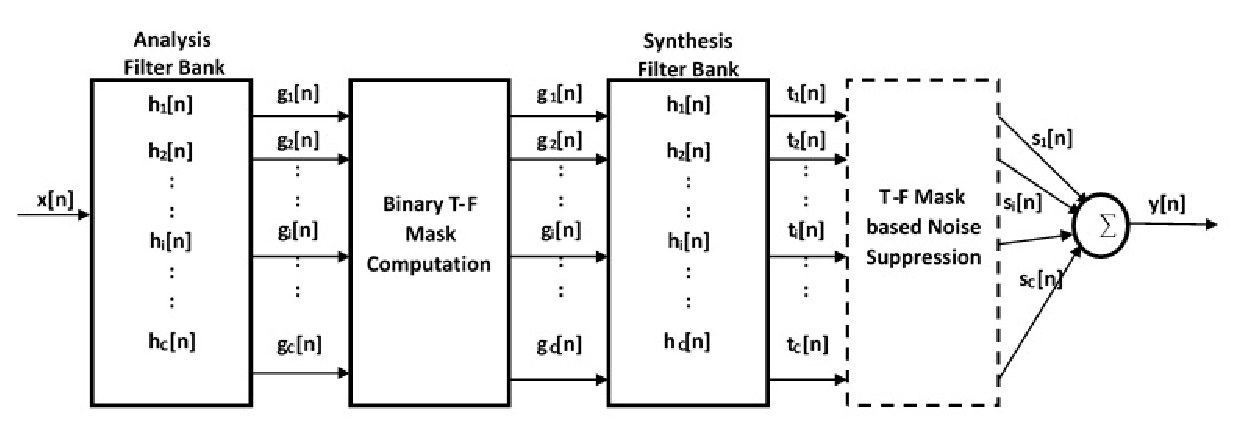
\includegraphics[width=\linewidth]{weintraub.eps}
  \caption{Block Diagram of Typical Speech Separation System}
  \label{fig:speech_production}
\end{figure}

\subsection{Speech Analysis}
The first step in the typical monaural speech separation system is the speech analysis. In which speech, noise and noisy speech will be decomposed into various sub-bands and each sub-band into various T-F units using analysis filter bank. The analysis filter bank performs a FFT filtering of the input signal with the impulse response of the gammatone filter. The output of the analysis filter bank gi[n] is given by
\begin{equation}
g_i{[n]} = x[n] * h_i{[n]};    1 \leq i \leq C.                                         
\label{eq3}
\end{equation}
where * indicates linear convolution, x[n] – input speech/noise/noisy speech and h\textsubscript{i}[n] - impulse response of the gammatone filter in i\textsuperscript{th} channel and C is the total number of channels.
\subsection{Binary T-F Mask Computation}
Computing binary mask is the computational goal of CASA. The speech signal which coming from the analysis filter bank is divided into various T-F units and the energy in each T-F unit is computed. Similarly, the energy of each noise T-F unit is also computed and is mathematically represented as 

\begin{equation}
Speech Energy : SE_{i,j}{[n]} = \sum_{m=jR}^{jR+L-1}(gS_i{[m]})^{2}                                            
\label{eq4}
\end{equation}
\begin{equation}
Noise Energy : NE_{i,j}{[n]} = \sum_{m=jR}^{jR+L-1}(gN_i{[m]})^{2}                                            
\label{eq5}
\end{equation}
where SE\textsubscript{i,j} - energy of speech signal and NE\textsubscript{i,j}   - energy of noise signal in i\textsuperscript{th}channel, j\textsuperscript{th}frame respectively, gS\textsubscript{i}  and gN\textsubscript{i}  are the filtered response of speech signal and noise signal in i\textsuperscript{th} channel respectively. L denotes the Frame length and Window shift R is given by R=L/2. Based on the energy values of speech and noise, the T-F Binary Mask is defined as 
\begin{equation}
M(t, f) = 
\begin{cases}
1&if \quad SE_{i,j}{[n]} > NE_{i,j}{[n]},\\
0&otherwise    
\label{eq6}
\end{cases}
\end{equation}
Where 1 indicates that the T-F unit is speech dominant and 0 indicates that the T-F unit is noise dominant.
\subsection{Speech Synthesis}
The final stage of typical monaural speech separation system is the speech synthesis by a synthesis filter bank. Synthesis filter bank performs the inverse operation of the analysis filter bank. Usually the coefficients in the synthesis filter bank will be the time reversed version of the analysis filter bank, but in this research work the synthesis filter bank uses the same coefficients as that of the analysis filter bank. Instead, the input and output of the synthesis filter bank is flipped in time, thus the original signal can be reconstructed. After estimating the ideal binary mask, the noisy speech signal g\textsubscript{i}[n] from each channel is flipped and then filtered using the synthesis filter bank. The filtered output is once again flipped and framed in to various T-F units by windowing technique. Finally, the computed ideal binary mask in the previous stage is multiplied to obtain the denoised speech. The mathematical expressions for the above steps in typical monaural speech separation system is given below
\begin{equation}
\begin{split}
k_i{[n]} &= f_i{[n]} * h_i{[n]};
\\
\indent &= \sum_{m=0}^{m=\infty}  f_i{[m]}h_i{[n-m]}                                    
\end{split}
\label{eq7}
\end{equation}
Here f\textsubscript{i}[n] = g\textsubscript{i}[-n].
\begin{equation}
s_{i,j}{[m]} = \sum_{m=jR}^{jR+L-1} t_i{[m]}p_{i,j}{[jR-m]}.                                            
\label{eq8}
\end{equation}
Where t\textsubscript{i}[n] = k\textsubscript{i}[-n]
\\
and p_{i,j}{[m]} =
\begin{cases}
w[n]\quad if \quad M(i,j)=1\\
0 \quad \quad otherwise                                          
\end{cases}

Here w[n] is the sliding cosine window which is defined as, 
\begin{equation}
w{[n]} =
\begin{cases}
1+ cos(2\pi (n-1)/L – \pi)/2 ;& 0 \leq n \leq L-1  \\
0 ;\quad\quad otherwise                                        
\label{eq9}
\end{cases}
\end{equation}
and finally the output from each channel s\textsubscript{i}[n] is added together to get the denoised output speech.
\begin{equation}
y{[n]} = \sum_{i=1}^{C} s_i{[n]}.                                            
\label{eq10}
\end{equation}
\section{Proposed Monaural Speech Separation System}
The proposed monaural speech separation system uses the same structure as that of the typical speech separation system except for the change in order of operation. The proposed model of monaural speech separation system is shown in Figure 2. In which, the IBM computed after the analysis filter bank is pre multiplied with the noisy speech signal and then sent to the synthesis filter bank. On multiplying the mask with the noisy speech signal many noise dominant frame will be made to zero. This makes the synthesis filter bank to reconstruct the speech signal with less amount of time as compared to the typical CASA speech separation system. 
\begin{figure}[t]
  \centering
  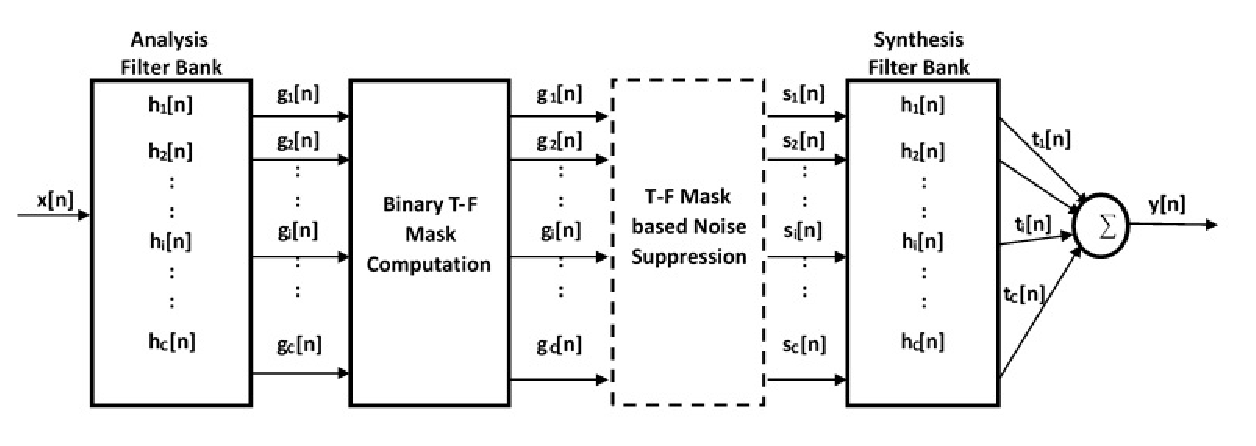
\includegraphics[width=\linewidth]{proposed.eps}
  \caption{Block Diagram of Proposed Speech Separation System}
  \label{fig:speech_production}
\end{figure}
The mathematical expression of the proposed system for speech resynthesis is shown below
\begin{equation}
s_{i,j}{[m]} = \sum_{m=jR}^{jR+L-1} g_i{[m]}p_{i,j}{[jR-m]}.                                            
\label{eq11}
\end{equation}
where p\textsubscript{i,j}{[m]} =
\begin{cases}
w[n] \quad ;M(i,j)=1\\
0 \quad ;M(i,j)=0                                          
\end{cases}
\\R=L/2 and w[n] is the sliding cosine window.\\
In the speech synthesis, the signal s\textsubscript{i}[n] (decomposed speech signal after mask multiplication) is flipped and convolved with the impulse response of the gammatone filter.
\begin{equation}
\begin{split}
k_i{[n]} &= f_i{[n]} * h_i{[n]};
\\
\indent &= \sum_{m=0}^{m=\infty}  f_i{[m]}h_i{[n-m]}                                    
\end{split}
\label{eq12}
\end{equation}
Here f\textsubscript{i}[n] = s\textsubscript{i}[-n].
\\The output of the synthesis filter bank from each channel k\textsubscript{i}[n] is once again flipped and added together to get the denoised output speech y[n]
\begin{equation}
y{[n]} = \sum_{i=1}^{C} t_i{[n]}.                                            
\label{eq13}
\end{equation}
where t\textsubscript{i}[n] = k\textsubscript{i}[-n]
\section{Experimental Results and Discussion}
The performance of the typical and the proposed CASA based speech separation systems is evaluated using the IEEE speech database [18] and Noisex-92 [19] noises. Both the systems were implemented in Matlab and tested using the Computer with the following specifications:\\
Intel® Core™ i5-3210M CPU@2.50Ghz, RAM: 4.00GB, 64- bit operating System, Windows 10 Home edition.\\
MATLAB Version: R2015a. \\
The design specification of the Gammatone analysis and synthesis filter bank is given below
\begin{table}[th]
  \caption{Filter Bank Specifications}
  \label{tab:word_styles}
  \centering
  \begin{tabular}{|c|c|c|}
    \hline
    \textbf{Parameters}        & \textbf{Typical}                            & \textbf{Proposed}\\
															 & \textbf{System} 													   & \textbf{System}\\
    \hline
    Order                      & $4$                                         & $4$    \\
		\hline
    Number of Channels         & $128$                                       & $128$  \\
		\hline
    Length of Impulse          & $1024$                                      & $1024$ \\
		Response									 &																						 &        \\
		\hline
  \end{tabular}
\end{table}


The performance of the proposed system evaluated in terms of speech quality and intelligibility. The quality of the enhanced speech by the proposed system is measured using Signal to Noise Ratio (SNR) improvement and intelligibility is measures using Short Time Objective Intelligibility (STOI) [20].\\
The SNR improvement is calculated using the following formula [21] [22]
\begin{equation}
SNR = 10×log(\frac{\sum_n S_{oneall}(n)^2}{\sum_n(S_{oneall}(n)-S_{out}(n))^2 })                                          
\label{eq14}
\end{equation}
where S\textsubscript{oneall}(n) - clean input speech signal and S\textsubscript{out}(n) -enhanced output speech signal. 
\\A clean speech signal from IEEE speech corpus is mixed with the babble noise and factory noise from Noisex-92 to obtain the noisy speech signal at SNRs in the range of -5dB to 15dB. This noisy speech is used to determine the SNR improvement and STOI of the proposed system at various input SNRs. The SNR improvement for the factory noise and babble noise is shown in Table 2 and Table 3. Similarly, the STOI value for the factory noise and babble noise is shown in Table 4 and Table 5. 
\begin{table}[th]
  \caption{SNR improvement of the proposed system for the factory noise at various input SNRs}
  \label{tab:word_styles}
  \centering
\begin{tabular}{|c|c|c|c|}
\hline
\textbf{Input} & \multicolumn{2}{|c|}{\textbf{Output SNR(dB)}}& \textbf{Improvement(dB)} 
& \cline{2-3}
\textbf{SNR(dB)}& \textbf{Typical} & \textbf{Proposed} & \\
 & \textbf{System} & \textbf{System} & \\
\hline
$-5$ & $7.6064$ & $7.9325$ & $0.3261$ \\
\hline
$0$ & $10.4869$ & $10.8704$ & $0.3835$ \\
\hline
$5$ & $13.9506$ & $14.3267$ & $0.3761$ \\
\hline
$10$ & $17.6725$ & $17.9212$ & $0.2487$ \\
\hline
$15$ & $21.5577$ & $21.7607$ & $0.2030$ \\
\hline
\textbf{Average} & $14.25482$ & $14.5623$ & $0.30748$ \\
\hline
\end{tabular}
\end{table}



\begin{table}[th]
  \caption{SNR improvement of the proposed system for the babble noise at various input SNRs}
  \label{tab:word_styles}
  \centering
\begin{tabular}{|c|c|c|c|}
\hline
\textbf{Input} & \multicolumn{2}{|c|}{\textbf{Output SNR(dB)}}& \textbf{Improvement(dB)} 
& \cline{2-3}
\textbf{SNR(dB)}& \textbf{Typical} & \textbf{Proposed} & \\
 & \textbf{System} & \textbf{System} & \\
\hline
$-5$ & $5.9454$ & $6.2761$ & $0.3307$ \\
\hline
$0$ & $8.4391$ & $8.8221$ & $0.3830$ \\
\hline
$5$ & $11.5351$ & $11.9661$ & $0.4310$ \\
\hline
$10$ & $15.0150$ & $15.2413$ & $0.2263$ \\
\hline
$15$ & $18.7670$ & $18.8917$ & $0.1247$ \\
\hline
\textbf{Average} & $11.94032$ & $12.23946$ & $0.29914$ \\
\hline
\end{tabular}
\end{table} 

From Table 2 and 3, it is observed that, the proposed system improves the output SNR with an average value of 0.30748 dB for factory noise and 0.29914 dB for babble noise respectively. This clearly shows that the proposed system improves the speech quality by improving the SNR.  The STOI [20] is used in this work as the intelligibility measure which is a simple and reliable objective measure based on short time segments. Generally, the value of STOI will be in the range of 0 to 1. The value of STOI is 1 means the enhanced speech is same as the clean speech and 0 means the enhanced speech has no correlation with the clean speech

\begin{table}[th]
  \caption{The STOI value of the proposed system for the factory noise}
  \label{tab:word_styles}
  \centering
\begin{tabular}{|c|c|c|c|}
\hline
\textbf{Input} & \multicolumn{2}{|c|}{\textbf{STOI}}& \textbf{Improvement} 
& \cline{2-3}
\textbf{SNR(dB)}& \textbf{Typical} & \textbf{Proposed} & \\
 & \textbf{System} & \textbf{System} & \\
\hline
-5 & 0.8011 & 0.8086 & 0.0075 \\
\hline
0 & 0.8629 & 0.8709 & 0.0080 \\
\hline
5 & 0.9016 & 0.9234 & 0.0218 \\
\hline
10 & 0.9367 & 0.9471 & 0.0104 \\
\hline
15 & 0.9595 & 0.9636 & 0.0041 \\
\hline
\textbf{Average} & 0.89236 & 0.90272 & 0.01036 \\
\hline
\end{tabular}
\end{table} 

\begin{table}[th]
  \caption{The STOI value of the proposed system for the babble noise}
  \label{tab:word_styles}
  \centering
\begin{tabular}{|c|c|c|c|}
\hline
\textbf{Input} & \multicolumn{2}{|c|}{\textbf{STOI}}& \textbf{Improvement} 
& \cline{2-3}
\textbf{SNR(dB)}& \textbf{Typical} & \textbf{Proposed} & \\
 & \textbf{System} & \textbf{System} & \\
\hline
-5 & 0.7754 & 0.7902 & 0.0148 \\
\hline
0 & 0.8048 & 0.8262 & 0.0214 \\
\hline
5 & 0.8560 & 0.8660 & 0.0100 \\
\hline
10 & 0.9060 & 0.9107 & 0.0047 \\
\hline
15 & 0.9487 & 0.9521 & 0.0034 \\
\hline
\textbf{Average} & 0.85818 & 0.86904 & 0.01086 \\
\hline
\end{tabular}
\end{table} 



Similarly, from Table 4 and Table 5, it observed that, the proposed system improves the STOI with an average value of 0.01036 for factory noise and 0.01086 for babble noise. This clearly shows that the proposed system improves the speech intelligibility by increasing the STOI value.\\
In addition to the above SNR improvement and STOI, computation time and throughput also considered to show the performance of the proposed system. Table 6 compares the computation time and throughput of the proposed system with the typical monaural speech separation system. 


\begin{table}[th]
  \caption{Comparison of computation time and throughput of the proposed speech separation system.}
  \label{tab:word_styles}
  \centering
  \begin{tabular}{|c|c|c|}
    \hline
    \textbf{Parameters}        & \textbf{Typical}                            & \textbf{Proposed}\\
															 & \textbf{System} 													   & \textbf{System}\\
    \hline
    Number of                  & $5768060928$                                & $5768060928$    \\
		Multiplications						 &																						 &				\\
		\hline
    Number of                  & $5759635712$                                & $5759635712$  \\
		Additions									 &																						 &        \\
		\hline
    Computational              & $3.32$                                      & $2.51$ \\
		Time(sec)									 &																						 &        \\
		\hline
		Throughput(samples				 &  $453$																			 & $517$   \\
		per sec)	  					     &  																					 &         \\
		\hline
  \end{tabular}
\end{table}


The number of multiplications and additions involved is calculated based on the number of frames, number of samples in each frame, the length of impulse response of Gamma tone filter and length of the input noisy speech signal. The number of multiplications and additions involved in both the systems are same. However, there is reduction of 24.4\% in the computation time of the proposed system which is evident from Table 6. It is mainly due to the number zeros introduced after multiplying the IBM with the T-F frames of noisy speech signal.  From Table 6 it is also observed that, the reduction of computation time leads to 14.13 \% improvement of throughput.
\section{Conclusion}
This research work proposed a new method for speech resynthesis in monaural speech separation system without compromising on the quality and intelligibility of the enhanced speech. The proposed method improves the speech quality and intelligibility with minimal computational delay and higher throughput by changing the order of operation. The proposed system requires the knowledge of clean speech and noise to compute the IBM, which is in general not feasible for practical applications. This research work focuses this issue and propose a new method to determine IBM without the knowledge of noise in future.


\bibliographystyle{IEEEtran}



 \begin{thebibliography}{9}

\bibitem[1]{Weintraub}
M.\ Weintraub,
"A theory and computational model of auditory monaural sound separation",
\textit{Ph.D. dissertation,Dept. Elect. Eng., Stanford Univ., Stanford, CA, },  1985.
	
\bibitem[2]{Stevan}
Stevan F.\ Boll,
"Suppression of acoustic noise in speech using spectral subtraction",
\textit{IEEE Transactions on Acoustics, Speech and Signal Processing}, vol.~2, no.~2, pp.~113-120, Apr 1989.

\bibitem[3]{Ephraim}
Y.\ Ephraim and H.\ L.\ Trees, "A signal subspace approach for speech enhancement", \textit{IEEE Trans. Speech Audio Processing}, Vol. ~3, pp. ~251-266, Jul 1995.     

\bibitem[4]{Sameti}
Sameti H, Sheikhzadeh H, Deng L, Brennan RL, "HMM based strategies for enhancement of speech signals embedded in nonstationary noise", \textit{IEEE Transactions on speech and audio processing}, Vol. ~6, Issue. ~5, pp. ~445-455, Sep 1998.

\bibitem[5]{Sameti}
J.\ Jensen, J.\ H.\ L.\ Hansen,  "Speech enhancement using a constrained iterative sinusoidal model", \textit{IEEE Transactions on speech and audio processing}, Vol. ~9, Issue. ~7, pp. ~731-740, Oct 2001.

\bibitem[6]{Jihen}
Jihen Zeremdini, Mohamed Anouar Ben Messaoud and Aicha Bouzid, "A comparison of several computational auditory scene analysis (CASA) techniques for monaural speech segregation", \textit{Brain Informatics}, Vol. ~2, Issue. ~3, pp. ~155-166, Sept 2015.

\bibitem[7]{wangbrown}
D.\ L.\ Wang, G.\ J.\ Brown, "Fundamentals of Computational Auditory Scene Analysis", in \textit{Computational Auditory Scene Analysis, D.L Wang and G.J Brown, Wiley-IEEE Press}, pp. ~1-38, 2006.           

\bibitem[8]{Harish}
N.\ Harish Kumar, R.\ Rajavel, "Monaural speech separation system based on optimum soft mask", \textit{IEEE Int. Conf. on Computational Intelligence and Computing Research}, Dec 2014. 

\bibitem[9]{Mane}
V.\ A.\ Mane, Prof.\  Dr.\ S.\ B.\ Patil, “Survey of Methods and challenges in Computational Auditory sense analysis”, \textit{ International Journal of Innovative Research in Electrical, Electronics, Instrumentation and Control Engineering}, Vol. ~4, Issue. ~9, Sept 2016.            

\bibitem[10]{sshobha}
S.\ Shoba, R.\ Rajavel, "Adaptive energy threshold for monaural speech separation", \textit{International Conference on Communication and Signal Processing}, 6-8 April 2017.

\bibitem[11]{Abrar}
Abrar Hussain, Kalaivani Chellappan, Siti Zamratol M, "Single Channel Speech Enhancement Using Ideal Binary Mask Technique Based On Computational Auditory Scene Analysis", \textit{Journal of Theoretical and Applied Information Technology}, Vol. ~91, No. ~1, Sept 2016.         

\bibitem[12]{Shobha}
S.\ Shoba, R.\ Rajavel, "Image processing techniques for segments grouping in monaural speech separation", \textit{Circuits, Systems, and Signal Processing (Springer), Published online - Dec 2017}, “https://doi.org/10.1007/s00034-017-0728-x”.         

\bibitem[13]{Wang}
D.\ L.\ Wang, "Time–Frequency Masking for Speech Separation and Its Potential for Hearing Aid Design", \textit{Trends in Amplification}, Vol. ~12, pp. ~332-353, Dec 2008.         

\bibitem[14]{Hu}
G Hu, D Wang, "Monaural speech segregation based on pitch tracking and amplitude modulation", \textit{IEEE Transactions on Neural Networks}, Vol. ~15, Issue. ~5, pp. ~1135-1150, Sept 2004.         

\bibitem[15]{hofmann}
V.\ Hofmann, "Frequency analysis and synthesis using a Gammatone filter bank", \textit{Acta Acustica united with Acustica}, Vol. ~88, pp. ~433 – 442, Jan 2002.        

\bibitem[16]{Patterson}
R.\ D.\ Patterson, I. Nimmo-Smith, J. Holdsworth, P. Rice, "An efficient auditory filterbank based on the gammatone function", \textit{MRC Applied Psych. Unit. 2341}, 1988.    

\bibitem[17]{Lawrence}
Lawrence R.\ Rabiner, Ronald W. Schafer, "Time Domain Methods for Speech Processing", in \textit{Theory and Applications of Digital Speech Processing,Lawrence R. Rabiner, Ronald W. Schafer, Pearson Education, Prentice Hall}, pp. ~287-379, 2011.            

\bibitem[18]{Rothauser}
E.\ H Rothauser et al, "IEEE recommended practice for speech quality measurements", \textit{IEEE Transactions on Audio and Electroacoustics}, Vol. ~17, pp. ~225–246, Sept 1969.        

\bibitem[19]{Noisex}
Noisex-92. "http://www.speech.cs.cmu.edu/comp.speech/Section1\\/Data/noisex.html", 2014.           

\bibitem[20]{Cees}
Cees H.\ Taal, Richard C.\ Hendriks, Richard Heusdens, and Jesper Jensen, "An algorithm for intelligibility prediction of time frequency weighted noisy speech", \textit{IEEE Transactions on Audio, Speech and Language Processing}, Vol. ~19, No. ~7, pp. ~2125-2136, Sept 2011.            

\bibitem[21]{Ke}
Ke Hu and DeLiang Wang, "An Unsupervised Approach to Cochannel Speech Separation", \textit{IEEE Transactions on Audio, Speech and Language Processing}, Vol. ~21, No. ~1, Jan 2013.                     

\bibitem[22]{Masoud}
Masoud Geravanchizadeh and Reza Ahmadnia, "Monaural Speech Enhancement Based On Multi-threshold Masking", \textit{In Blind Source Separation, G.R. Naik, W. Wang, Springer Berlin Heidelberg}, pp. ~369-393, 2014.

\bibitem[23]{Belhidi}
Belhedi Wiem, Ben Messaoud Mohamed Anouar, Bouzid Aichl, "Time-Frequency Masks for Monaural Speech Separation: A Comparative Review", \textit{7th International Conference on Sciences of Electronics, Technologies of Information and Telecommunications (SETIT)}, 2016.





 \end{thebibliography}















\end{document}
